\documentclass[11pt,onecolumn]{article}
\usepackage {graphicx}
\usepackage{latex8}
\usepackage{times}
\usepackage{amsmath}
\usepackage{amssymb}
\usepackage{amsthm}
\bibliographystyle{latex8}


\begin{document}
%
% paper title
% can use linebreaks \\ within to get better formatting as desired
\title{CloudProtect: A Middleware for Managing Privacy in Cloud Applications}


% author names and affiliations
% use a multiple column layout for up to two different
% affiliations

\author{
 Prosunjit Biswas\\
 \textit{UTSA}
}


% make the title area
\maketitle


\begin{abstract}
Cloud computing applications have increased significantly in recent years due to improved
accessibility, availability and services at reduced costs. Examples of such
services include Google Calendar, Microsoft HealthVault, and Yahoo Briefcase. In
such services, the service provider provides the storage as well as the web application
that utilizes the storage. Despite their benefits however, these services present
significant security and privacy risks to their users. Users data is exposed to both
outsider and insider attacks, and users dont have any control over the security and
privacy management of the data. We propose CloudProtect, a middleware that sits
between the client and service provider applications empowering users with the ability
to manage their security and privacy needs for these cloud applications. The middleware
enables the tradeoff analysis between data privacy, usability, and efficiency.
We implemented CloudProtect and adapted it to work with Google Calendar, Google
Docs, and Gmail. Our experimental results highlight the feasibility of the approach.
\end{abstract}



\Section{Introduction}
With the advances of the web and cloud computing technologies, we are undergoing a
paradigm shift in how we manage our data and build applications. A variety of enduser
applications that let users manage their emails, documents, healthcare data etc.,
are available today over the cloud. The application-as-a-service model offers numerous
advantages to end-users – e.g., 24/7 availability, accessibility from anywhere/anytime,
lower cost etc. Examples of such services include calendar applications [1],
document management applications [2], database as a service applications
[7, 8], personal health record services to name a few. These applications are
available to users either free of charge or on pay-peruse basis. Instead of acquiring and
installing the applications on their machines, users can access them from anywhere
at any time simply through a browser based interface. As a result, large volumes of
personal and organizational data is migrating to the cloud at an amazing pace.

\paragraph{}

The fundamental issue is that once the data is stored at the service provider, users
do not have any control over how it is used or who accesses it on the service provider
side. As a consequence, this lack of mechanisms for enabling end-users to control
security of their data at the service-provider is one of the primary limitations to the
adoption of cloud applications.  Furthermore, the security mechanisms followed by them
remain vulnerable to insider attacks. Many surveys [5] have revealed that concerns
of security and privacy are the primary barriers to adoption of cloud computing by
governmental, healthcare, and financial institutions. Even if the service providers
themselves were fully trusted, since the cloud applications authenticate end-users
through login credentials, the data stored within the applications are vulnerable to
miscreants who steal such credentials and masquerade as data owners.
\paragraph{}

In this thesis, we propose an extendible middleware called CloudProtect, the goal
of which is to enable user-driven application level data to be stored on the service
provider side in encrypted form. CloudProtect empowers the end users to add an extra
layer of protection to their own data.  To limit such overheads, CloudProtect maintains a
policy that dictates which data is stored in plaintext and which is stored encrypted at
the server. Such a policy, learnt from user interaction with the application, supports
a tradeoff between costs/overhead incurred and the amount of (duration for which)
sensitive data is exposed in plain text to the server. The policies learnt by Cloud-
Protect are based on user-specified parameters that capture the degree of tolerance a
user has to increased overheads as well as to potential information breach and are,
furthermore, subject to human-override. Additionally, CloudProtect facilitates key
management and secure sharing of encrypted data.

\paragraph{Contribution}

\begin{enumerate}
\item
 We propose CloudProtect, a middleware framework that mediates between users
and the cloud applications providers to enable privacy management services.
The framework includes a data model and function model for describing the
cloud applications and a policy model for expressing confidentiality policies.

\item
 CloudProtect enables the automatic tradeoff of privacy, usability, and efficiency.
Privacy is measured in terms of the number privacy violations, usability by
the number of interruptions, and efficiency through the cost associated with
the executions of operations on transformed objects. Given the set of objects
that have been stored so far in the database, the tradeoff is achieved by generalizing/
relaxing the policies so that the number of interruptions and/or costs
associated with the operations are below some thresholds.

\end{enumerate}



\Section{Related Work}
CloudProtect is related to recently proposed system Silverline [4] that also aimed
to support encrypting user data in cloud applications 1. Silverline introduced the
concept of functional encryption wherein the system identifies all data items that can
be encrypted in a manner that is transparent to the application. It uses dynamic program
analysis to identify functionally encryptable data in a cloud-based application
and proposes an encryption key assignment and sharing solution that enables people
\paragraph{}
Another closely related work is the technical report presented in [6]. Like CloudProtect,
this report considers a middleware based approach for providing privacy management
in cloud applications. The middleware is implemented as a proxy that can
process both HTTP and HTTPS requests. Sharing the encryption keys is also performed
via email messages that cannot be accessed by the cloud application servers.
In addition to randomized encryption for strong protection, deterministic encryption
is used to support search on the encrypted data, with lesser security. This work however
differs from CloudProtect in a number of ways. (1) It does not abstract out the
data and the functionality of the cloud applications into a general framework, which
can be adapted for any application. (2) It does not provide an expressive policy-based
data encryption mechanism such as CloudProtect, which can be used to selectively
encrypt the data. All data is encrypted without considering the implication in terms
of efficiency. (3) Encryption naturally increases the computation and communication
overheads of the cloud applications. Unlike CloudProtect where these overheads can
be reduced though policy rebalancing, this approach does not address this problem.
The PrivatePond system [2] considers the problem of outsourcing storage and search
to an untrusted server. Like CloudProtect, the search engine functionality of the server
is preserved. The main idea is that search can be carried out using a secured index.
A simple indexable representation of data is presented. For the security analysis
two attack models are considered; one attack is on a single indexable representation
9

\Section{Proposed Method}
As mentioned before, the goal of CloudProtect is to enable users to selectively decide
how to protect their data through transformations, and alert the users through
interruptions when certain operations cannot be queried out or incur high cost due
to some transformations. Deciding how data is to be transformed (or not be transformed)
is achieved through privacy policies. Anytime the representation of a data
item is changed to enable the execution of an operation, an exception to the policy
is generated. These exceptions correspond to the privacy violations and increase
proportionally with the interruptions.


The CloudProtect framework shown in  \ref{Fig1}  involves three entities: user, cloud application (web
client, web server, DB), and privacy middleware. Figure 3.1 depicts the high-level
design of the framework. The user interacts with the web server through the web
client, implemented as a web browser application, to store and retrieve data from
the DB. The Privacy Middleware performs the tasks of encrypting the data to store
on the server and decrypting the data retrieved from the server according to the
user policies. The life-cycle of the framework comprises three phases: initialization,
operational, and policy rebalancing. In the following, each of these phases is described in details.

\begin{figure}
  \centering
  % Requires \usepackage{graphicx}
  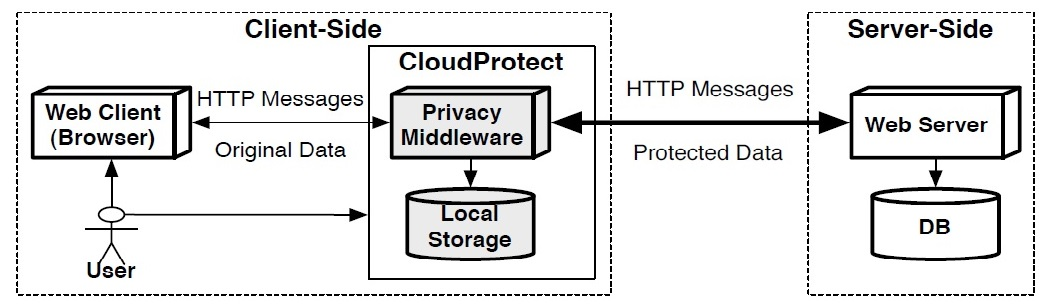
\includegraphics[width=0.75\textwidth]{cloudprotect.jpg}
  \caption{Cloud Protect Framework}
  \label{Fig1}
\end{figure}



\subsection{Initialization Phase}
The initialization phase includes the registration of the cloud applications to be serviced
by CloudProtect, the definition of confidentiality policies, and setting up system
parameters. Each application that is supported in CloudProtect needs to be registered
one time, during which, the data model and the function model are created and stored
in the local storage. Using the data model, a user can define confidentiality policies
or just use the default policy of encrypting everything strongly.
\subsubsection{Data Model}
We take an object oriented approach to modeling the user data in an application.
The data object is defined by a set of attributes and each data item is an instance
of this object. More formally, let us model the data stored at the database as a
set of n multidimensional objects, (o1, o2, · · · , on), where each object oi is a tuple of
k attributes \{A1, A2, · · · , Ak\}. Each attribute Ai is defined as a tuple of the form 	 $\langle name, value, type \rangle$	. We denote the set of these attributes by o.A where $\mid o.A\mid$ = n,
$n \ge 1$. The attribute name Ai.name and the attribute type Ai.type are determined by
the server and the attribute value Ai.value is the user or system data (to be made more
precise below). The attribute name Ai.name is the unique identifier of the attribute.
The attribute type Ai.type can be a simple data type such as “string”, “integer”,
“double”, and “boolean”, or a complex data type such as“text file”, “image file”,
“video file”, and “sound file”. For instance, in Google Calendar, there is an object
corresponding to every event and its fields such as “what”, “when”, and “where”,
comprise the set of attributes. Similarly, in Google Docs, a file can be the object o
and the file content, the creation date and the author, the attributes of the object o.
\subsubsection{Functional Model}
We model a cloud application services/functionality as a set of m functions
{F1, F2, · · · , Fm}, which operate on a subset of the object attributes. F is similar in
spirit to a method in object oriented programming, which needs to be instantiated
with specific parameters at runtime. Given an instantiation of a function F and a set
of objects \{o1, o2, · · · , on\} on which F is applied to, there is a concept of dependence
between F and the objects. We say that F depends on an object o, iff F is operated
on at least one attribute of o. Hence, the normal execution of F depends on the
particular representations of the dependent attributes in o. On Google Calendar for
example, the successful execution of the function search on “where” depends only on
how this attribute is transformed not the others like “what” and “description”.

\subsubsection{Data Encryption}
CloudProtect’s protection mechanism consists of a library of type-specific transformation
techniques. It combines all the applicable rules to derive the appropriate
protection level for an attribute of an object. We use a tagging technique similar to
that used in XML, to embed the transformed data in the HTTP messages. The tags
show where the encrypted data starts and ends in both, an HTTP request and HTTP
response. This tagging technique is very useful for segmenting the transformed data
embedded in the server-response.



\Section{Performance}
The objectives of the experiments were to measure the performance of CloudProtect
as implemented and used for Google Calendar and Google Docs. We measured the
computation costs of the middleware in enforcing data confidentiality constraints by
encrypting and decrypting data objects, and the associated storage costs. In addition
to the basic experiments that compare the storage/computation tradeoffs, we analyzed
the two implemented algorithms (deterministic and randomized encryptions)
along the following dimensions: scalability, search performance, and content heterogeneity.
The scalability experiment investigated the behavior of the middleware in
terms of computation cost as the number of objects to encrypt and decrypt increases.
\paragraph{}
The search performance study focuses on the system performance in terms of query
execution over encrypted data. The content heterogeneity experiment explored how
the variation in the size of the objects affects the behavior of the middleware.
We used real data to drive the experiments on both Google Calendar and Google Docs.
For Google Calendar, we generated a number of events, with different sizes, ranging
approximately from 1KB to 20KB. For Google Docs, we selected also a number of
files of varying types (doc, excel, ppt, pdf, text) and sizes (from 28 KB to 4000 KB).
All experiments were executed on a MacBook Pro laptop machine.
Since the current implementation of the middleware utilizes only cryptographic algorithms
to protect the data, we use the time it takes for encryption and decryption
of the data and the extra storage needed by the encryption algorithms as the main
metrics for the experimental study.

\Section{Conclusion and Future Work}
Ensuring privacy of data in cloud applications, where service providers are not trusted
is challenging. The difficulty stems from the fact that service providers do not provide
any support for protecting users’ data. In this thesis, we propose CloudProtect, a
policy-based privacy middleware for supplementing existing cloud applications with
a mechanism for protecting users data, without any modification of these applications.
CloudProtect is intended to work with a variety of cloud applications where
one has no control over the server side functionality beyond what API’s may provide.
Such API’s often do not have any support for data confidentiality at all. We take
a more “pragmatic” approach to provisioning data confidentiality in cloud applications
- here data may be partially exposed as long as it does not violate the privacy
constraints. For example, the requirement that certain “attribute values not be exactly
determinable” can be a privacy constraint. Such an approach, which represents
a significant departure from prior work, has numerous advantages. In addition to improved efficiency, limited disclosure allows for “value-added” services that are key benefits of today’s personal data outsourcing services.


\begin{thebibliography}{1}
\small

\bibitem{IEEEhowto:kopka} Mihir Bellare, Thomas Ristenpart, Phillip Rogaway, and Till Stegers. Formatpreserving
encryption. In Selected Areas in Cryptography, pages 295–312, 2009.
 Lucas Ballard, Seny Kamara, and Fabian Monrose. Achieving efficient conjunctive
\bibitem{IEEEhowto:kopka} keyword searches over encrypted data. In ICICS, pages 414–426, 2005.
 Mihir Bellare, Alexandra Boldyreva, and Adam O’Neill. Deterministic and efficiently
searchable encryption. In CRYPTO, pages 535–552, 2007.

Hakan Hacig¨um¨us, Balakrishna R. Iyer, Chen Li, and Sharad Mehrotra. Executing
sql over encrypted data in the database-service-provider model. In SIGMOD
Conference, pages 216–227, 2002.
\bibitem{IEEEhowto:kopka} Yan-Cheng Chang and Michael Mitzenmacher. Privacy preserving keyword
searches on remote encrypted data. In ACNS, pages 442–455, 2005.
\bibitem{IEEEhowto:kopka} Hakan Hacig¨um¨us, Bijit Hore, Balakrishna R. Iyer, and Sharad Mehrotra. Search
on encrypted data. In Secure Data Management in Decentralized Systems, pages
383–425. 2007.
\bibitem{IEEEhowto:kopka} Craig Gentry. Fully homomorphic encryption using ideal lattices. In Michael
Mitzenmacher, editor, STOC, pages 169–178. ACM, 2009.
\bibitem{IEEEhowto:kopka} Krishna P. N. Puttaswamy, Christopher Kruegel, and Ben Y. Zhao. Silverline:
Toward data confidentiality in third-party clouds. In ACM Symposium on Cloud
Computing, October 2011.

\end{thebibliography}

\end{document}


